\PassOptionsToPackage{unicode=true}{hyperref} % options for packages loaded elsewhere
\PassOptionsToPackage{hyphens}{url}
%
\documentclass[]{article}
\usepackage{lmodern}
\usepackage{amssymb,amsmath}
\usepackage{ifxetex,ifluatex}
\usepackage{fixltx2e} % provides \textsubscript
\ifnum 0\ifxetex 1\fi\ifluatex 1\fi=0 % if pdftex
  \usepackage[T1]{fontenc}
  \usepackage[utf8]{inputenc}
  \usepackage{textcomp} % provides euro and other symbols
\else % if luatex or xelatex
  \usepackage{unicode-math}
  \defaultfontfeatures{Ligatures=TeX,Scale=MatchLowercase}
\fi
% use upquote if available, for straight quotes in verbatim environments
\IfFileExists{upquote.sty}{\usepackage{upquote}}{}
% use microtype if available
\IfFileExists{microtype.sty}{%
\usepackage[]{microtype}
\UseMicrotypeSet[protrusion]{basicmath} % disable protrusion for tt fonts
}{}
\IfFileExists{parskip.sty}{%
\usepackage{parskip}
}{% else
\setlength{\parindent}{0pt}
\setlength{\parskip}{6pt plus 2pt minus 1pt}
}
\usepackage{hyperref}
\hypersetup{
            pdftitle={TooDoot},
            pdfborder={0 0 0},
            breaklinks=true}
\urlstyle{same}  % don't use monospace font for urls
\usepackage{graphicx,grffile}
\makeatletter
\def\maxwidth{\ifdim\Gin@nat@width>\linewidth\linewidth\else\Gin@nat@width\fi}
\def\maxheight{\ifdim\Gin@nat@height>\textheight\textheight\else\Gin@nat@height\fi}
\makeatother
% Scale images if necessary, so that they will not overflow the page
% margins by default, and it is still possible to overwrite the defaults
% using explicit options in \includegraphics[width, height, ...]{}
\setkeys{Gin}{width=\maxwidth,height=\maxheight,keepaspectratio}
\setlength{\emergencystretch}{3em}  % prevent overfull lines
\providecommand{\tightlist}{%
  \setlength{\itemsep}{0pt}\setlength{\parskip}{0pt}}
\setcounter{secnumdepth}{0}
% Redefines (sub)paragraphs to behave more like sections
\ifx\paragraph\undefined\else
\let\oldparagraph\paragraph
\renewcommand{\paragraph}[1]{\oldparagraph{#1}\mbox{}}
\fi
\ifx\subparagraph\undefined\else
\let\oldsubparagraph\subparagraph
\renewcommand{\subparagraph}[1]{\oldsubparagraph{#1}\mbox{}}
\fi

% set default figure placement to htbp
\makeatletter
\def\fps@figure{htbp}
\makeatother


\title{TooDoot}
\date{}

\begin{document}
\maketitle

\hypertarget{funzionalitaux300-dellapplicazione}{%
\section{Funzionalità
dell'applicazione}\label{funzionalitaux300-dellapplicazione}}

\begin{itemize}
\tightlist
\item
  Creazione, modifica e rimozione delle attività
\item
  Personalizzazione dell'attività con aggiunta di descrizione, priorità,
  data, ora, liste e tag
\item
  Visualizzazione del calendario con relativa lista delle attività
  giornaliere
\item
  Visualizzazione dei grafici con percentuale e numero delle attività
  completate, con possibilità di selezione di data, liste e tag
\item
  Ricerca e filtraggio delle attività
\item
  Notifiche giornaliere per ogni attività da svolgere
\item
  Impostazione di priorità minima delle attività da visualizzare e di
  cui essere noticati
\item
  Salvataggio automatico dei task nel formato todo.txt
\item
  Caricamento di file todo.txt
\end{itemize}

\hypertarget{todo.txt}{%
\section{todo.txt}\label{todo.txt}}

L'applicazione non fa altro che interfacciarsi a un file di testo
formato \texttt{todo.txt}, che ha principalmente il vantaggio di essere
facilmente leggibile e di essere comodo per l'utente il quale può
leggerlo e modificarlo con un semplice file di testo (vedi:
\href{https://github.com/todotxt/todo.txt}{todo.txt format}). Inoltre in
questo modo è anche facile la sincronizzazione su più dispositivi,
perché si tratta solo di sincronizzare dei file di testo.

\begin{figure}
\centering
\includegraphics{https://raw.githubusercontent.com/todotxt/todo.txt/master/description.png}
\caption{Task in formato todo.txt}
\end{figure}

\hypertarget{componenti}{%
\section{Componenti}\label{componenti}}

\hypertarget{attivitaux300}{%
\subsection{Attività}\label{attivitaux300}}

Le attività o task sono il componente principale dell'applicazione, ed è
formata dalle seguenti proprietà:

\begin{itemize}
\tightlist
\item
  \textbf{Nome:} Titolo dell'attività
\item
  \textbf{Stato:} Tiene conto se l'attività é completata o meno
\item
  \textbf{Descrizione:} Informazioni aggiuntive sull'attività
\item
  \textbf{Priorità:} Importanza dell'attività, è associata una priorità
  ad ogni lettera dalla A (priorità alta) alla Z (priorità bassa)
\item
  \textbf{Data:} Giorno in cui deve essere svolta l'attività
\item
  \textbf{Tempo:} Ora in cui deve essere svolta l'attività
\item
  \textbf{Liste (o contesti):} Corrisponde al posto o alla situazione in
  cui viene svolta l'attività
\item
  \textbf{Tag:} Qualunque tipo di tag relativo all'attività
\end{itemize}

Tutte queste proprietà (a parte lo stato) possono essere nulle

\begin{figure}
\centering
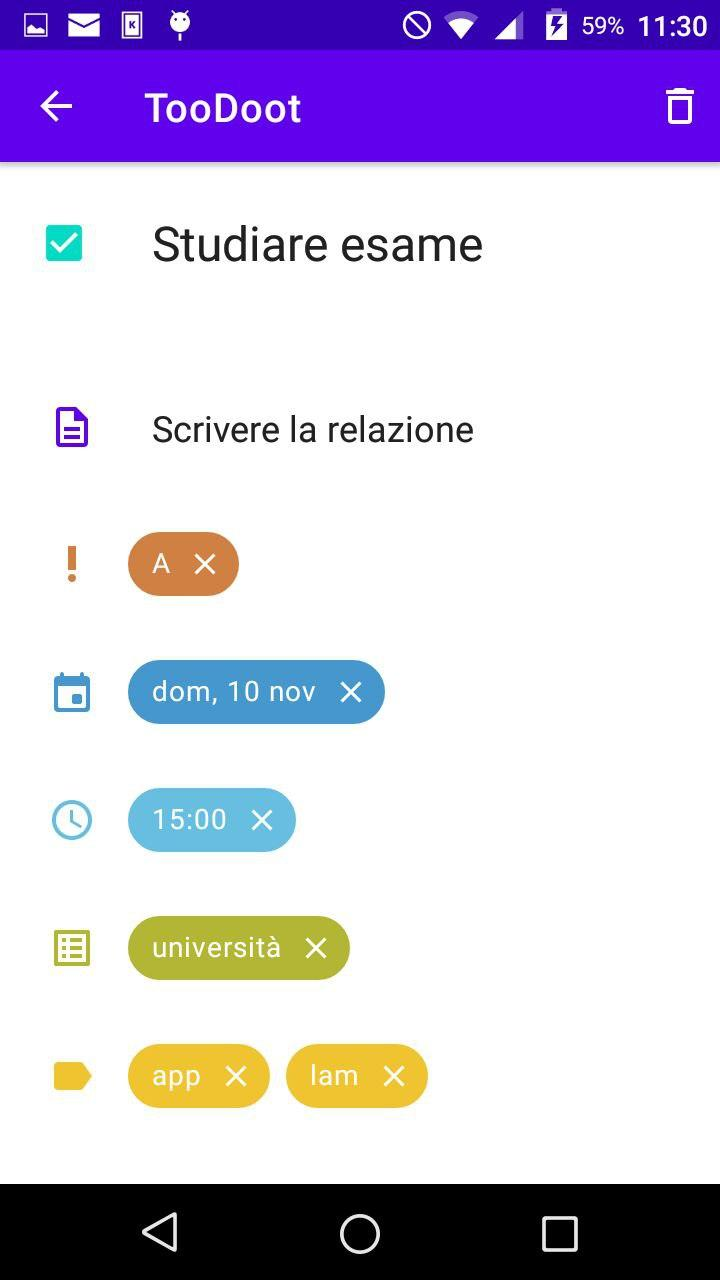
\includegraphics[width=0.3\textwidth,height=0.1\textheight]{./img/schermata_edit.jpg}
\caption{Questa schermata verrà salvata come la seguente linea del file
todo.txt: x (A) 2019-11-10 2019-11-10 Studiare esame
desc:Scrivere\_la\_relazione time:15:00 due:2019-11-10 +app +lam
@università}
\end{figure}

\hypertarget{liste-e-tag}{%
\subsection{Liste e Tag}\label{liste-e-tag}}

Le liste e i tag sono gestiti come stringhe, liberamente eliminabili e
aggiungibili nell'attività. Ogni attività avrà zero o più liste o zero o
più tag a seconda di quello che selezionerà l'utente. A livello
implementativo non c'è differenza tra liste e tag (se non che sono
separati) quindi spetterà all'utente scegliere come utilizzarli per
l'uno o per l'altro tipo; ma si consiglia di utilizzare le liste come
contesti in cui viene realizzata l'attività, mentre i tag come qualsiasi
tipo di parole chiave ad essa associate.

\hypertarget{notifiche}{%
\subsection{Notifiche}\label{notifiche}}

L'applicazione permette di ricevere notifiche relative alle attività,
infatti ad ogni notifica è associato un'attività che deve essere ancora
completata. Nelle impostazioni l'utente può selezionare l'orario di
arrivo delle notifiche, e ogni giorno a quell'ora gli verranno inviate
le notifiche di tutte le attività non ancora completate previste per
quella giornata. Le notifiche vengono, poi, inviate quando si fa il boot
del dispositivo. Inoltre l'utente può impostare una priorità minima per
cui un'attività venga notificata.

\begin{figure}
\centering
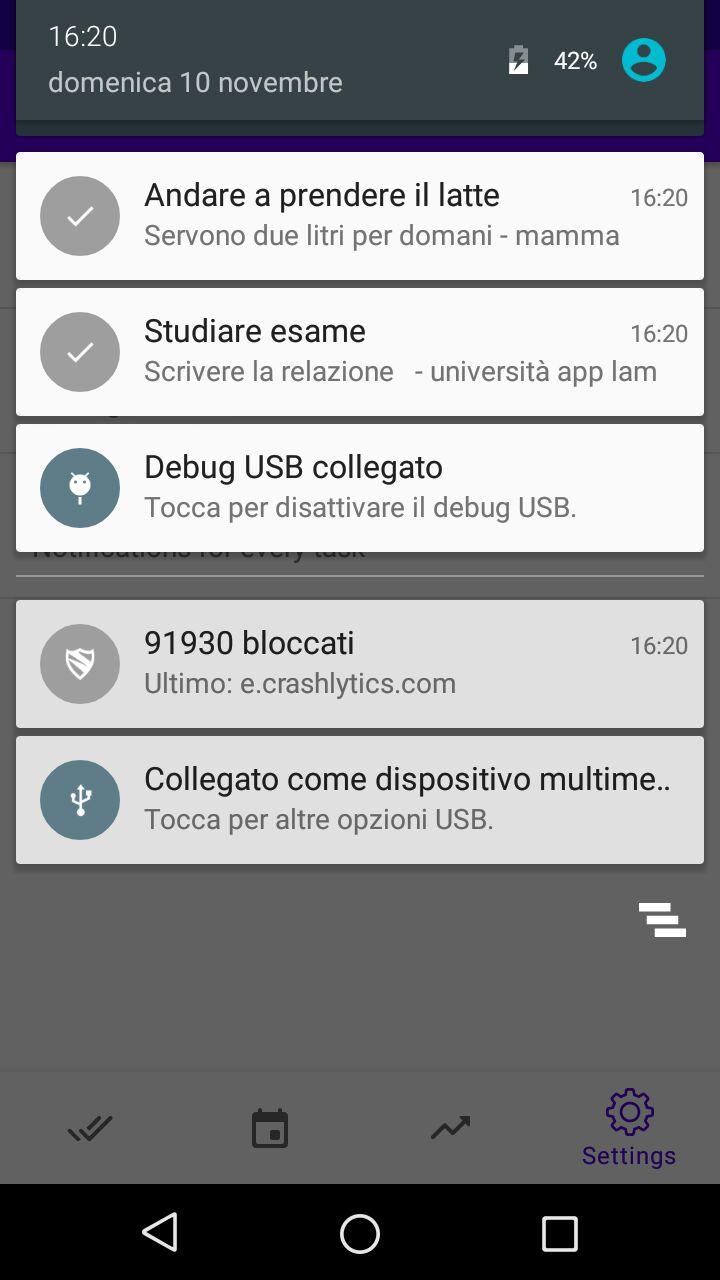
\includegraphics[width=0.3\textwidth,height=0.1\textheight]{./img/notifiche.jpg}
\caption{Notifiche}
\end{figure}

\hypertarget{schermate}{%
\section{Schermate}\label{schermate}}

Graficamente l'applicazione è gestita da quattro schermate (lista delle
attività, calendario, grafici e impostazioni) selezionabili da un bottom
menu, più una schermata (modifica attività) che viene aperta quando
viene cliccata un'attività della lista

\hypertarget{lista-delle-attivitaux300}{%
\subsection{Lista delle attività}\label{lista-delle-attivitaux300}}

Questa schermata mostra l'elenco di tutte le attività, e per ogni
attività vengono mostrate tutte le sue proprietà (a parte la
descrizione).

L'ordine della attività é determinato dalle seguenti proprietà:

\begin{itemize}
\tightlist
\item
  Vengono visualizzati le attività non completate e prima di quelle
  completate
\item
  A parità di stato vengono visualizzate in ordine crescente di data e
  ora
\item
  Se due attività hanno anche la stessa data e ora allora viene
  visualizzate in ordine decrescente di priorità
\item
  Qualora tra due attività tutti i parametri precedenti dovessero essere
  uguali vengono mostrati in ordine descrescente di creazione
\end{itemize}

Nella schermata ad ogni singola attività è stata aggiunto lo swipe:

\begin{itemize}
\tightlist
\item
  Swipe a destra: viene segnata l'attività come completata
\item
  Swipe a sinistra: viene posticipata l'attività (il valore è
  determinato da un dialog)
\end{itemize}

In questa schermata è anche possibile aggiungere le attività È possibile
filtrare le attività tramite la ricerca, che oltre al nome dell'attività
cercherà tutti i vari campi

\begin{figure}
\centering
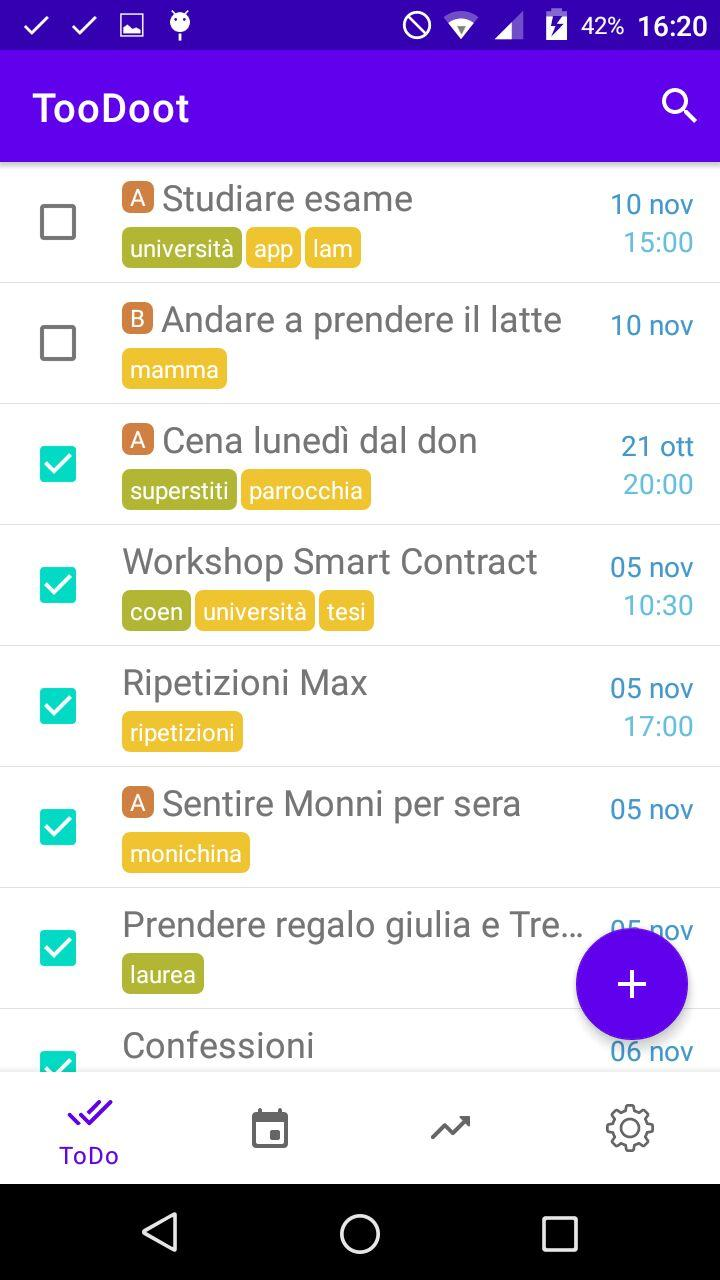
\includegraphics[width=0.3\textwidth,height=0.1\textheight]{./img/schermata_todo.jpg}
\caption{Schermata lista delle attività}
\end{figure}

\begin{figure}
\centering
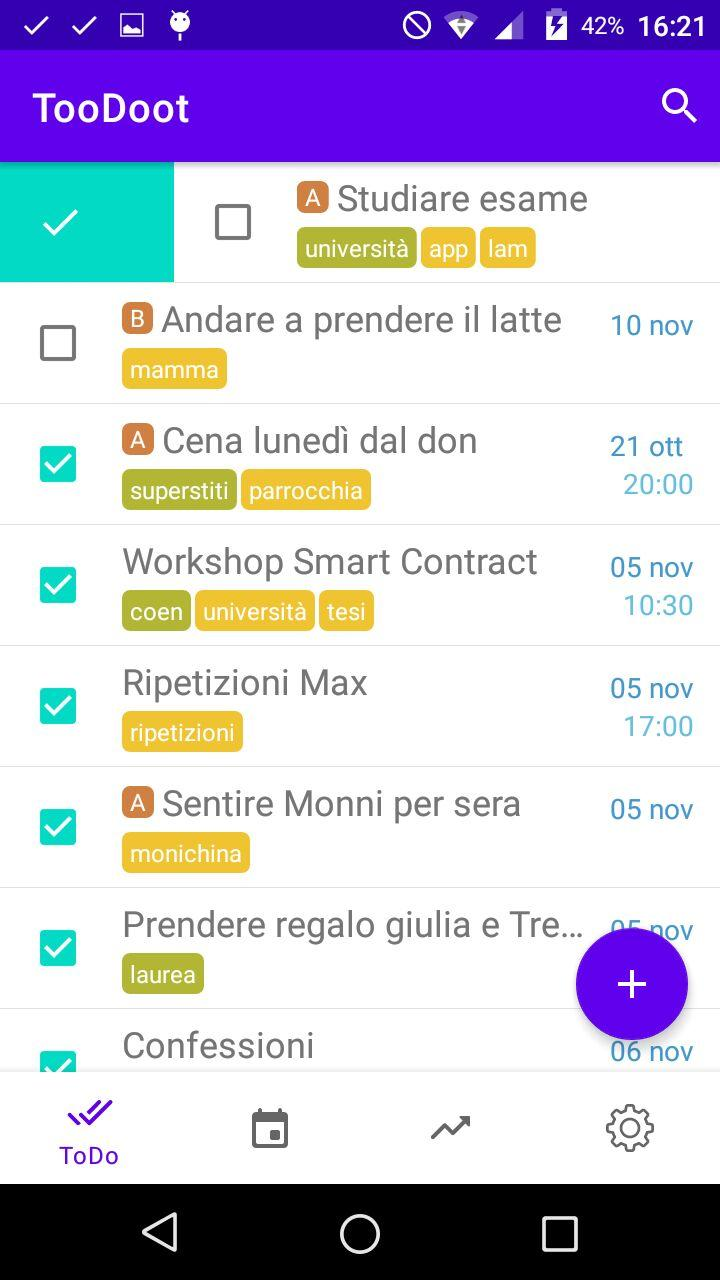
\includegraphics[width=0.3\textwidth,height=0.1\textheight]{./img/swipe_dx.jpg}
\caption{Swipe a destra}
\end{figure}

\begin{figure}
\centering
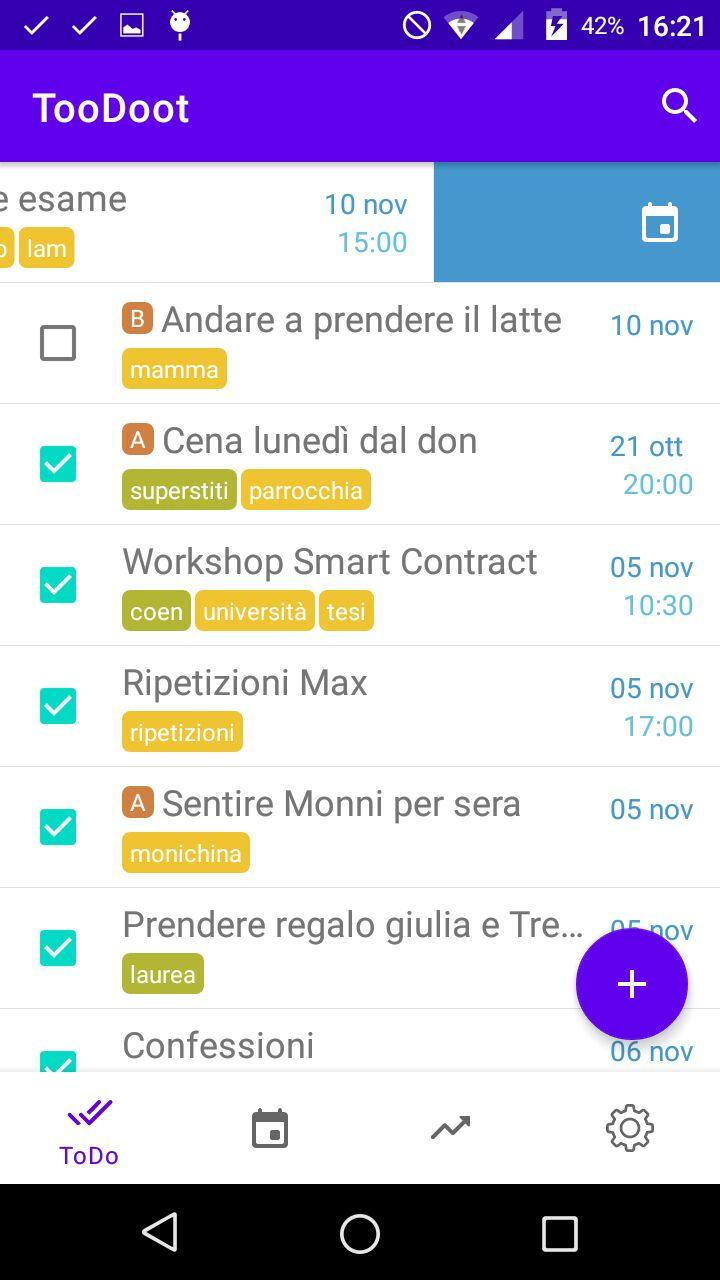
\includegraphics[width=0.3\textwidth,height=0.1\textheight]{./img/swipe_sx.jpg}
\caption{Swipe a sinistra}
\end{figure}

\hypertarget{calendario}{%
\subsection{Calendario}\label{calendario}}

La schermata a calendario consente di selezionare una data in modo da
mostrare l'elenco delle attività previste per quella determinata data,
esattamente come è mostrato nella lista delle attività. Alla data sul
calendario non sempre corrisponde la data dell'attività infatti
quest'ultima potrebbe non essere specificata: in questo caso come data
dell'attività verrà considerata la data di completamento, se anche
quest'ultima non è specificata (basta che l'attività non sia completata)
viene considerata come data dell'attività la data del giorno attuale.

\begin{figure}
\centering
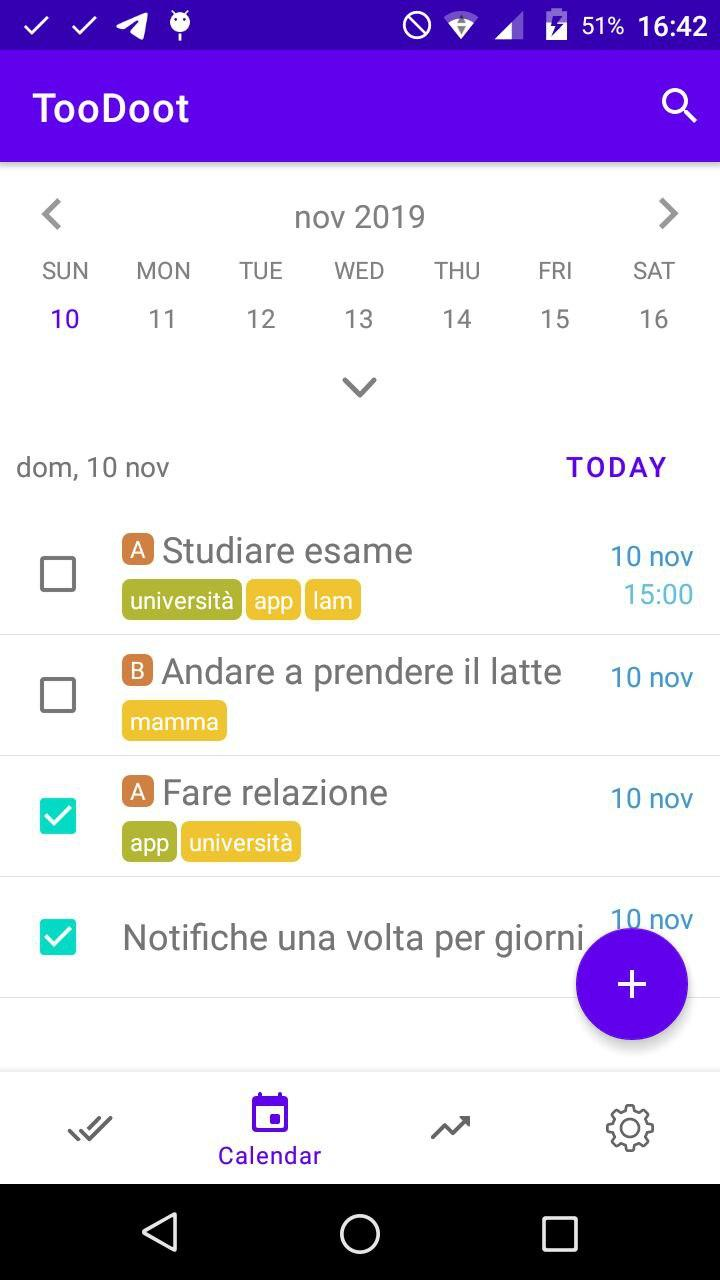
\includegraphics[width=0.3\textwidth,height=0.1\textheight]{./img/calendario_compatto.jpg}
\caption{Calendario compatto}
\end{figure}

\begin{figure}
\centering
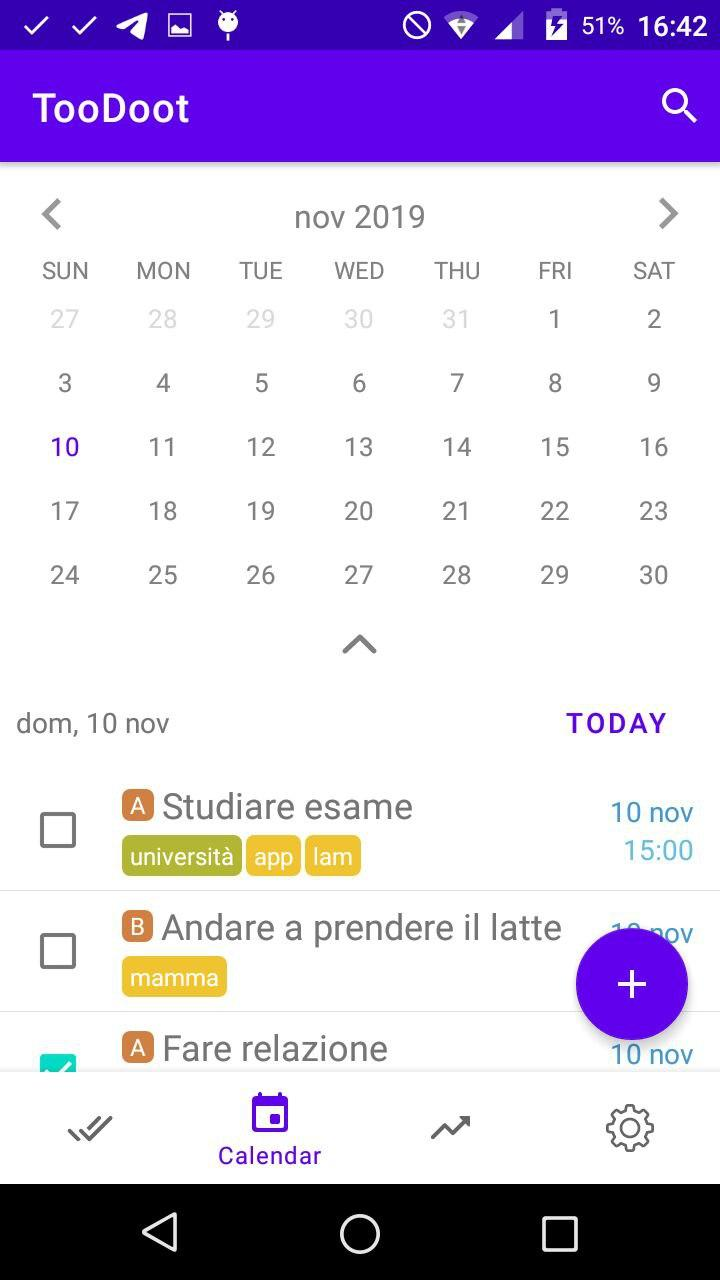
\includegraphics[width=0.3\textwidth,height=0.1\textheight]{./img/calendario_esteso.jpg}
\caption{Calendario esteso}
\end{figure}

\hypertarget{grafici}{%
\subsection{Grafici}\label{grafici}}

In questa schermata vengono mostrati due tipi di grafici: il diagramma a
torta e il diagramma a linee. È possibile selezionare una lista o un tag
in modo da avere le specifiche solo per un determinato tipo di attività

\hypertarget{grafico-a-torta}{%
\subsubsection{Grafico a torta}\label{grafico-a-torta}}

In questo grafico viene mostrata la percentuale dei task completati
rispetto ai task ancora da completare. È possibile selezionare un
intervallo di tempo, per decidere quali attività prendere in
considerazione:

\begin{itemize}
\tightlist
\item
  Tutte
\item
  Giornaliere
\item
  Settimanali
\end{itemize}

\hypertarget{grafico-a-linee}{%
\subsubsection{Grafico a linee}\label{grafico-a-linee}}

A differenza del grafico precedente prende in considerazione solo le
attività completate, queste verranno sommate in modo da avere un totale
per l'intervallo di tempo specificato, che può essere:

\begin{itemize}
\tightlist
\item
  Giornaliero
\item
  Settimanale
\item
  Mensile
\end{itemize}

\begin{figure}
\centering
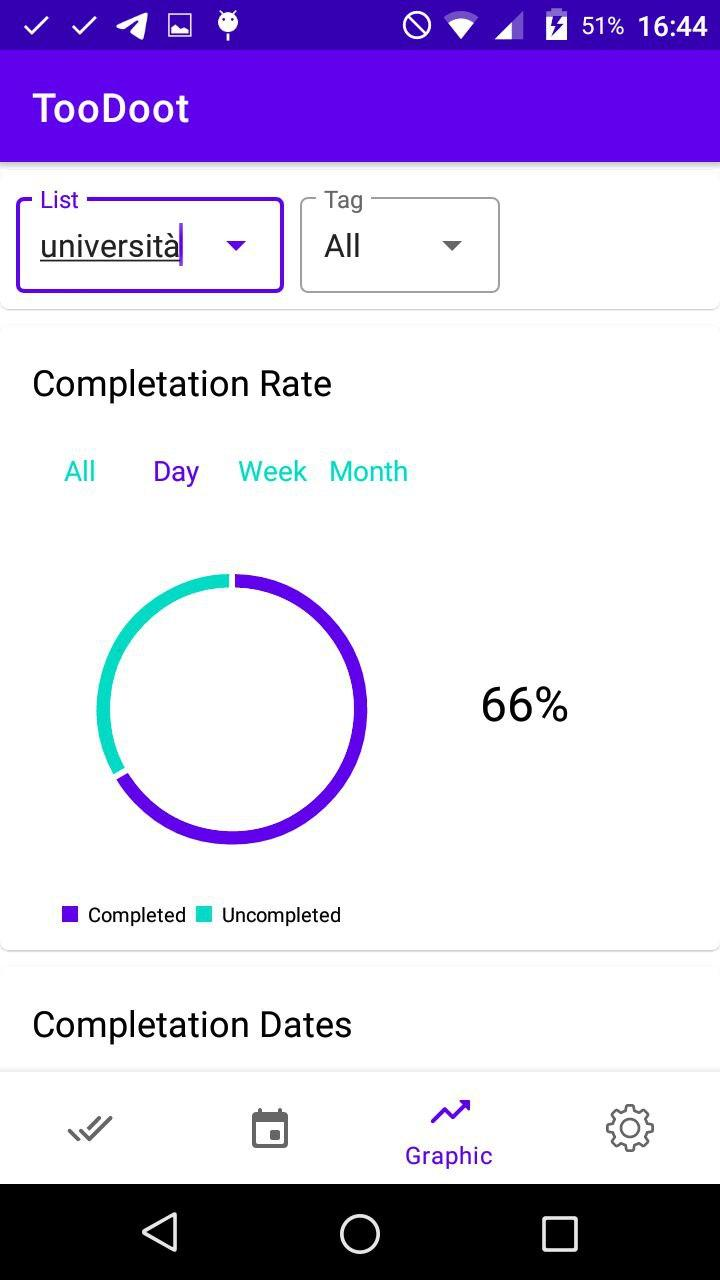
\includegraphics[width=0.3\textwidth,height=0.1\textheight]{./img/grafico_torta.jpg}
\caption{Grafico a torta}
\end{figure}

\begin{figure}
\centering
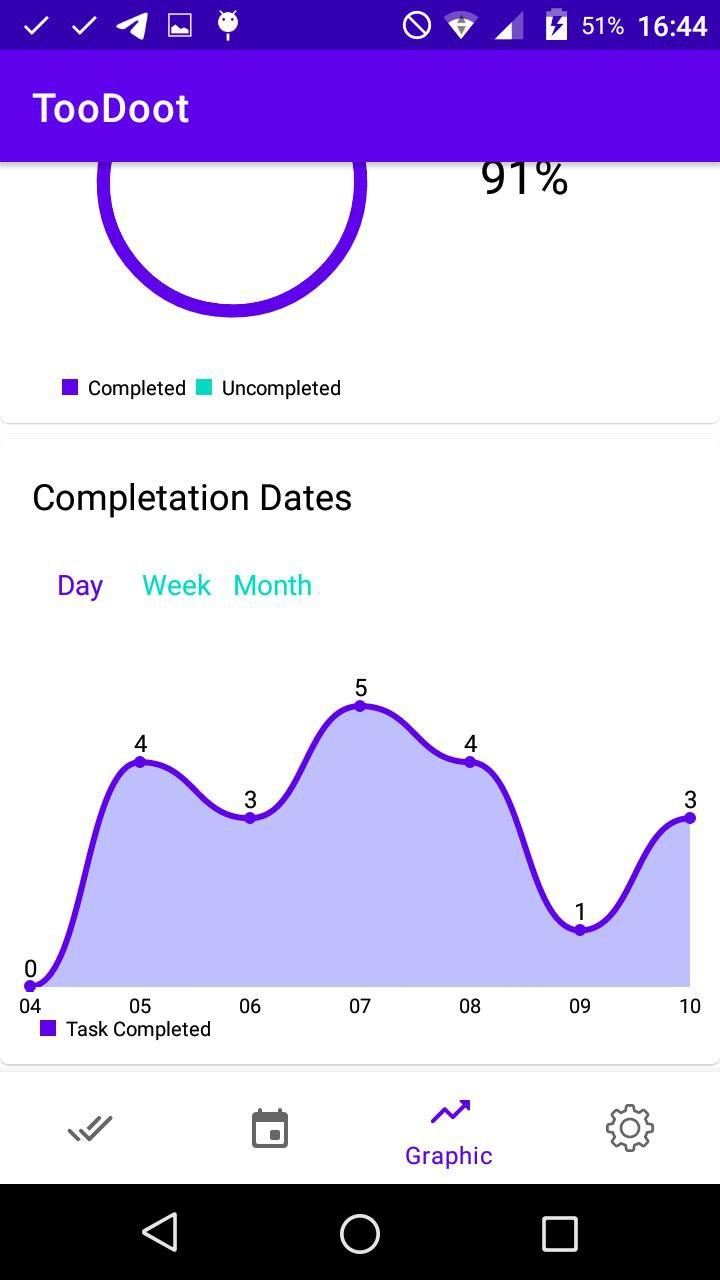
\includegraphics[width=0.3\textwidth,height=0.1\textheight]{./img/grafico_linee.jpg}
\caption{Grafico a linee}
\end{figure}

\hypertarget{impostazioni}{%
\subsection{Impostazioni}\label{impostazioni}}

La schermata delle impostazioni permette di modificare le preferenze
dell'applicazione, è possibile:

\begin{itemize}
\tightlist
\item
  Caricare un altro \texttt{todo.txt} presente nella memoria del
  dispositivo
\item
  Cambiare cartella del \texttt{todo.txt}, quindi spostare quest'ultimo
\item
  Impostare la priorità minima per le applicazioni
\item
  Modificare l'ora di ricevimento giornaliero delle notifiche
\end{itemize}

\begin{figure}
\centering
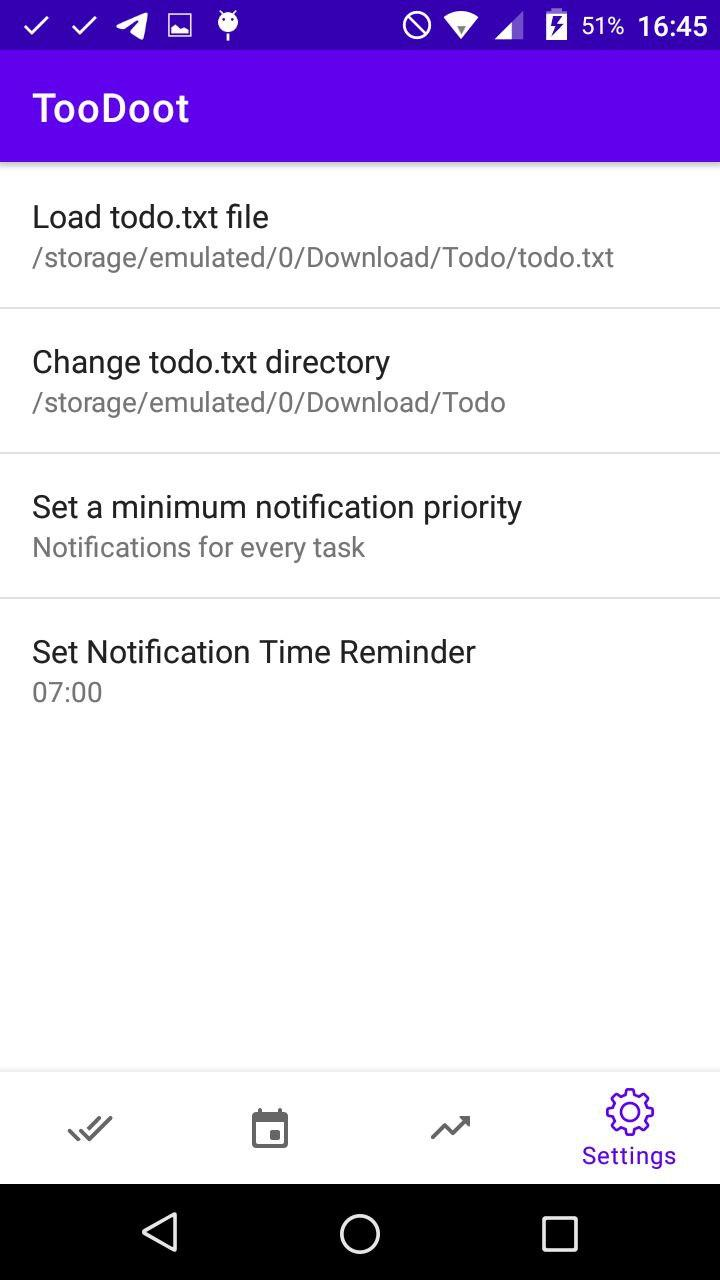
\includegraphics[width=0.3\textwidth,height=0.1\textheight]{./img/impostazioni.jpg}
\caption{Impostazioni}
\end{figure}

\hypertarget{modifica-attivitaux300}{%
\subsection{Modifica attività}\label{modifica-attivitaux300}}

In questa schermata è possibile modificare -quindi aggiungere, cambiare
o rimuovere i campi- o rimuovere un'attività.

\begin{figure}
\centering
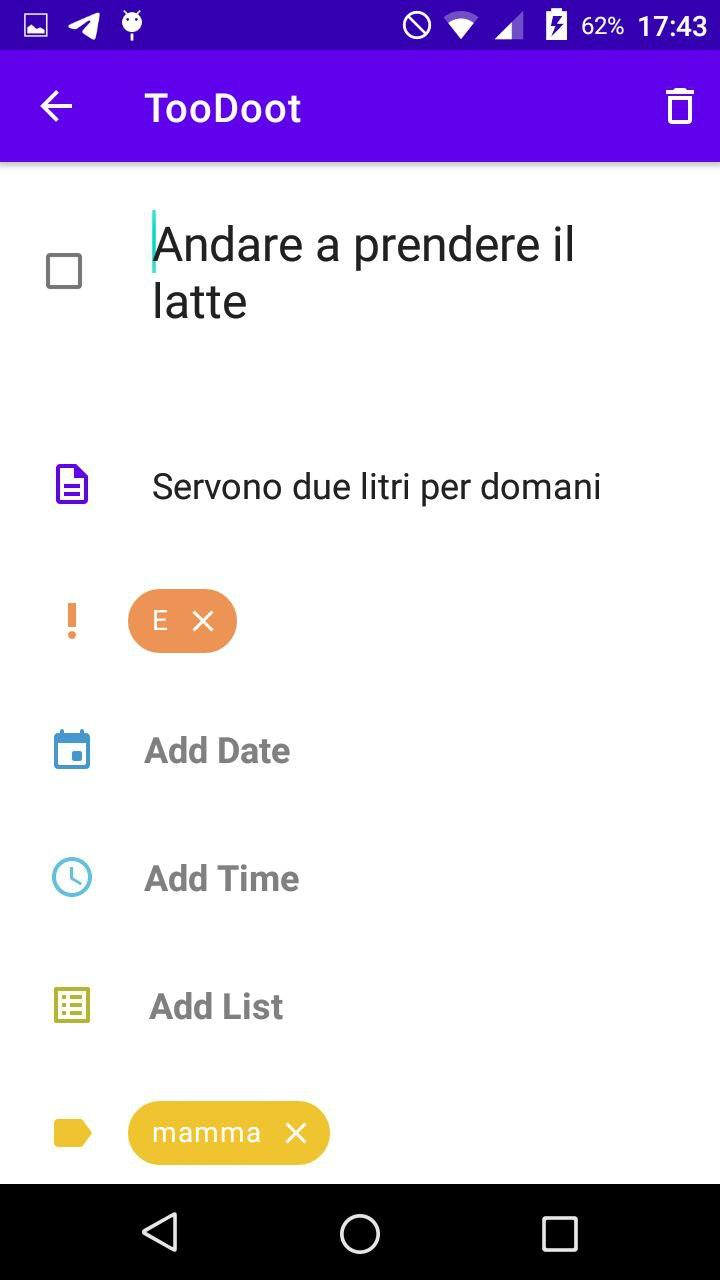
\includegraphics[width=0.3\textwidth,height=0.1\textheight]{./img/schermata_modifica.jpg}
\caption{Schermata modifica attività}
\end{figure}

\hypertarget{dialog}{%
\section{Dialog}\label{dialog}}

Ci sono diversi tipi di dialog che vanno in supporto alle varie
schermate

\hypertarget{aggiungi-attivitaux300}{%
\subsection{Aggiungi attività}\label{aggiungi-attivitaux300}}

In questo dialog è possibile aggiungere un nuovo task, specificando,
oltre al nome, i relativi campi che si vuole inserire

\begin{figure}
\centering
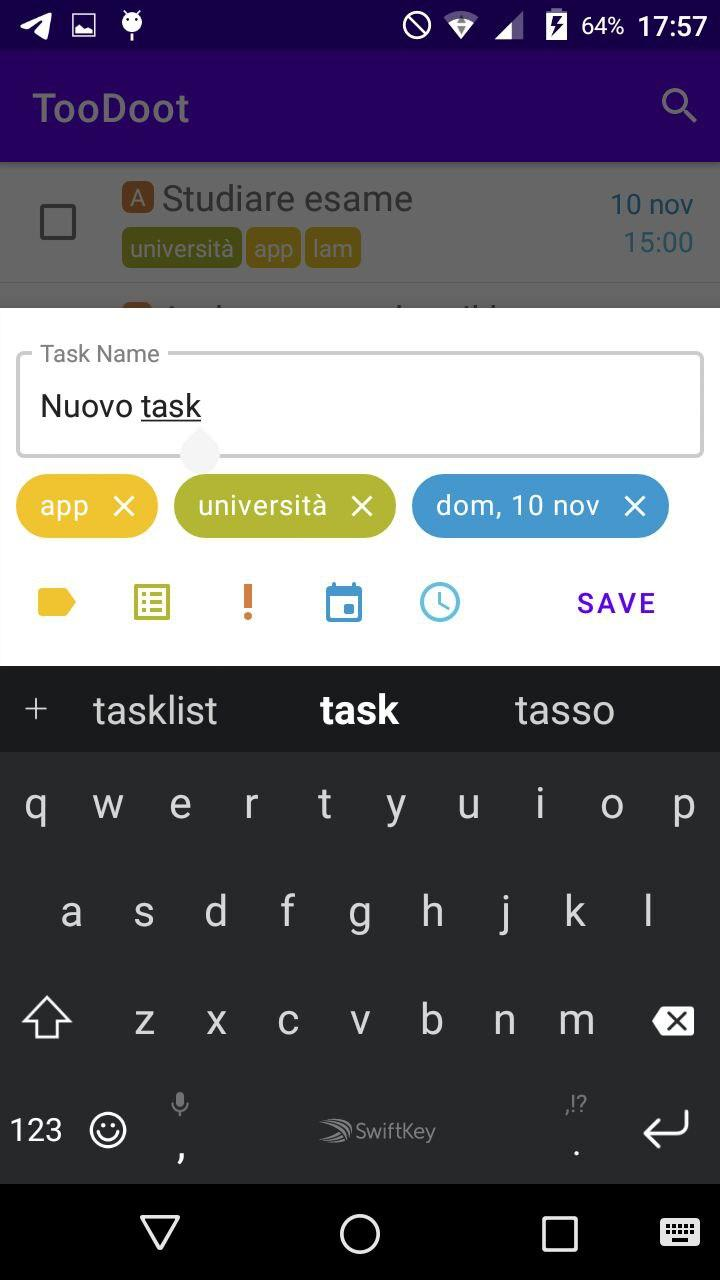
\includegraphics[width=0.3\textwidth,height=0.1\textheight]{./img/dialog_aggiungi.jpg}
\caption{Dialog aggiungi attività}
\end{figure}

\hypertarget{dialog-di-modifica}{%
\subsection{Dialog di modifica}\label{dialog-di-modifica}}

Quando si vuole inserire o modificare un nuovo campo viene mostrato il
dialog relativo, sono quindi:

\begin{itemize}
\tightlist
\item
  \textbf{Priorità:} Consiste in un picker di lettere: la lettera
  selezionata sarà la priorità
\item
  \textbf{Data:} Consiste in un date picker
\item
  \textbf{Ora:} Consiste in un time picker
\item
  \textbf{Liste e Tag:} Ci sono due dialog separati ma uguali,
  permettono di aggiungere nuove liste o tag, o di selezionarne tra
  quelli già esistenti
\end{itemize}

\begin{figure}
\centering
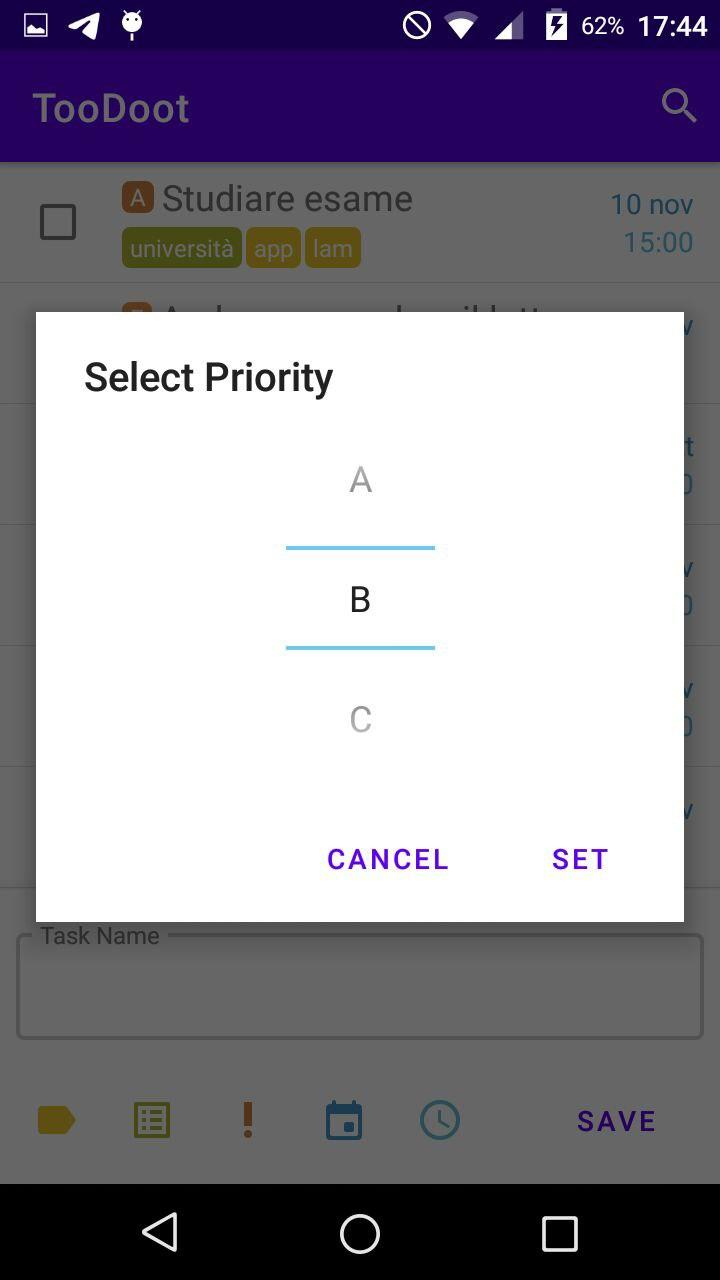
\includegraphics[width=0.3\textwidth,height=0.1\textheight]{./img/dialog_priority.jpg}
\caption{Dialog seleziona priorità}
\end{figure}

\begin{figure}
\centering
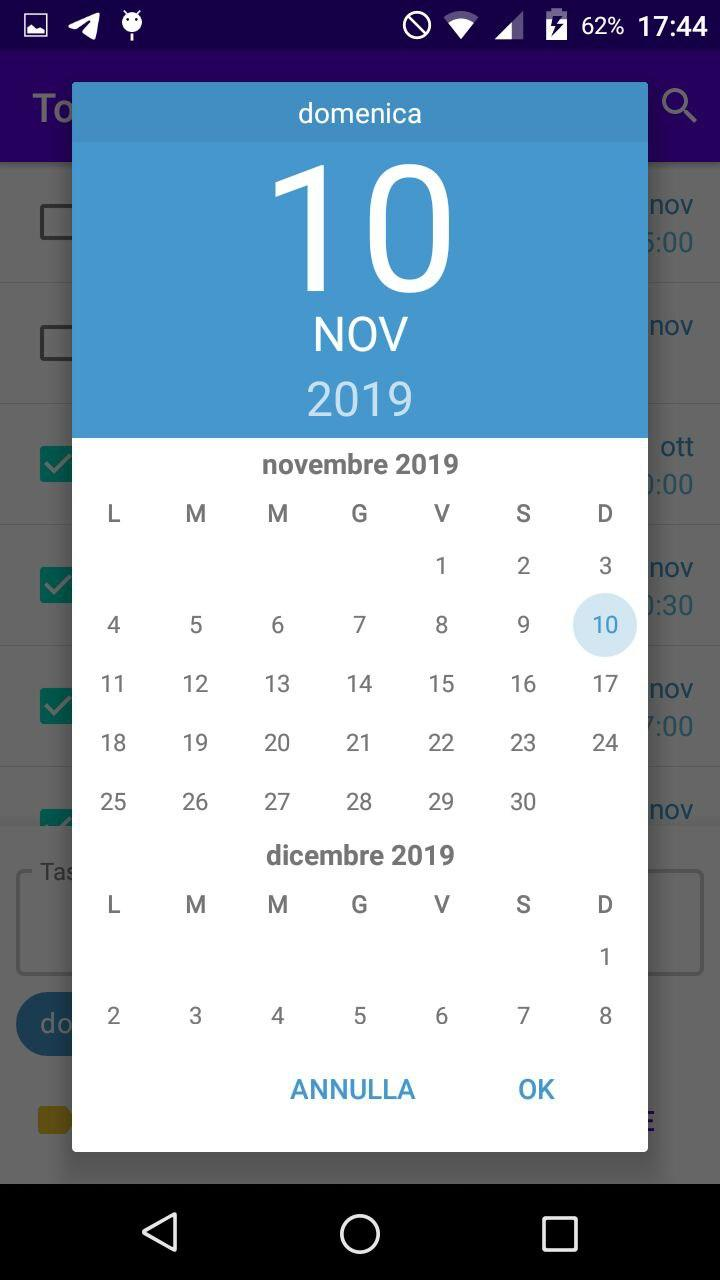
\includegraphics[width=0.3\textwidth,height=0.1\textheight]{./img/dialog_data.jpg}
\caption{Dialog seleziona data}
\end{figure}

\begin{figure}
\centering
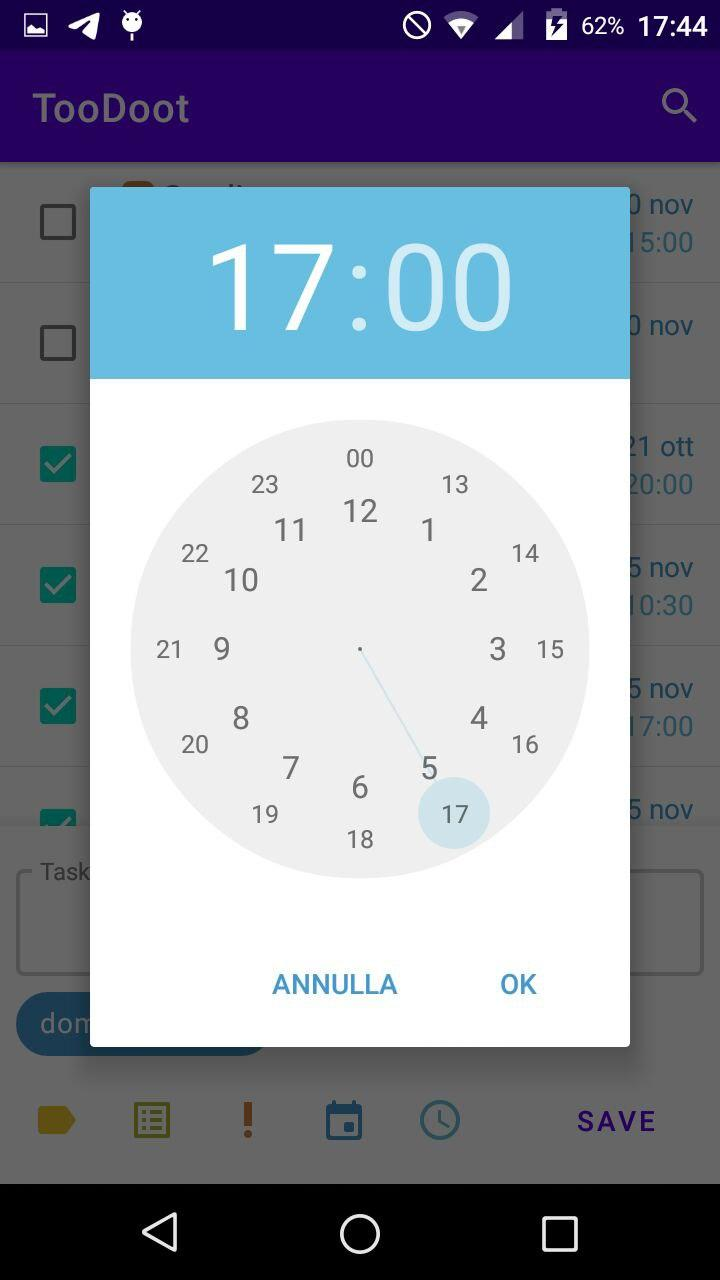
\includegraphics[width=0.3\textwidth,height=0.1\textheight]{./img/dialog_picker.jpg}
\caption{Dialog seleziona ora}
\end{figure}

\begin{figure}
\centering
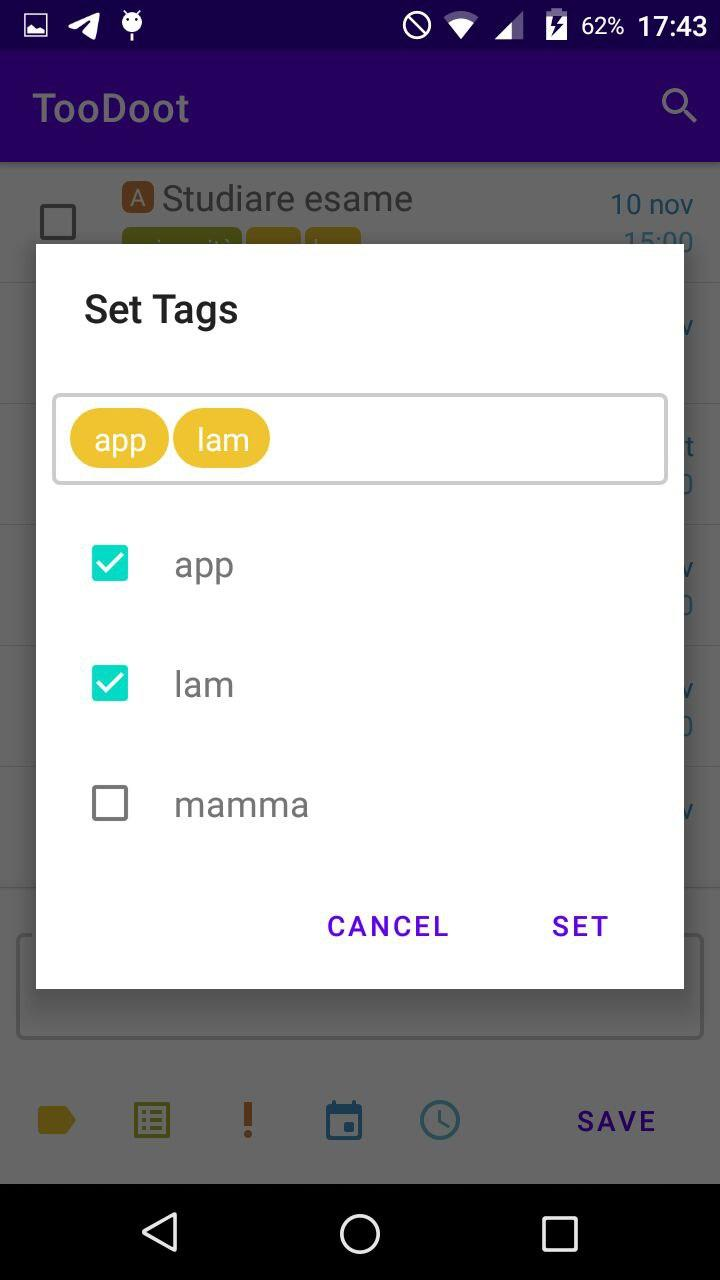
\includegraphics[width=0.3\textwidth,height=0.1\textheight]{./img/dialog_task.jpg}
\caption{Dialog aggiungi tag}
\end{figure}

\hypertarget{posticipa-attivitaux300}{%
\subsection{Posticipa attività}\label{posticipa-attivitaux300}}

Dopo lo swipe a sinistra nella lista delle attività viene mostrato
questo dialog che permette all'utente di posticipare l'attività in una
data a sua scelta

\begin{figure}
\centering
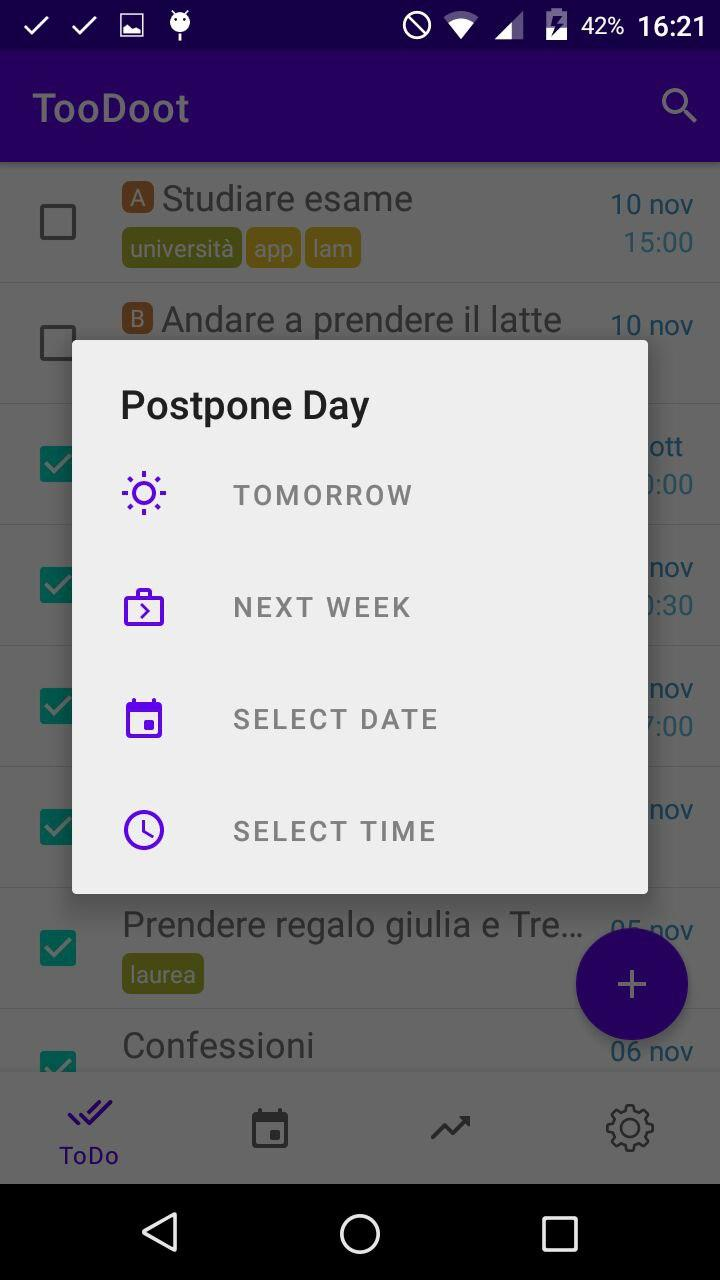
\includegraphics[width=0.3\textwidth,height=0.1\textheight]{./img/postpone_dialog.jpg}
\caption{Dialog posticipa}
\end{figure}

\hypertarget{implementazione}{%
\section{Implementazione}\label{implementazione}}

\hypertarget{interfaccia-utente}{%
\subsection{Interfaccia utente}\label{interfaccia-utente}}

A livello implementativo l'interfaccia utente consiste in un'activity
principale (\texttt{MainActivity}), contenente un bottom menu, la top
bar con la ricerca e il container il quale viene riempito dai vari
fragment (̀\texttt{TodoFragment}, \texttt{CalendarFragment},
\texttt{GraphicFragment} e \texttt{SettingFragment}) ogni volta che
viene selezionato un'icona nel bottom menu.

\begin{verbatim}
@Override
public boolean onNavigationItemSelected(@NonNull MenuItem item) {

    switch (item.getItemId()) {
        case R.id.navigation_todo: {
            makeSearchVisible(true);
            fragment = new TodoFragment(
                Task.getSavedTasks(getApplicationContext()));
            todoFragment = (TodoFragment)fragment;
            break;
        }
        case R.id.navigation_calendar: {
            makeSearchVisible(true);
            fragment = new CalendarFragment();
            calendarFragment = (CalendarFragment)fragment;
            break;
        }
        case R.id.navigation_graphic: {
            makeSearchVisible(false);
            fragment = new GraphicFragment();
            break;
        }
        case R.id.navigation_settings: {
            makeSearchVisible(false);
            fragment = new PreferencesFragment(MainActivity.this);
            break;
        }
    }
    return loadFragment(fragment);
}
\end{verbatim}

\hypertarget{task}{%
\subsection{Task}\label{task}}

I task vengono creati dell'\texttt{AddTaskFragment}, modificati e
eliminati nel \texttt{EditTaskActivity} e visualizzati nel
\texttt{TodoFragment}. In quest'ultimo alla lista di attività è
associata una \texttt{RecyclerView} che con il relativo
\texttt{TaskAdapter}, chefornisce una view per ogni task. Ogni modifica
da parte dell'utente alla lista di attività consiste in una chiamata al
\texttt{TodoFragment} che chiama il suo \texttt{TaskAdapter} che esegue
poi l'operazione sulla lista.

Tutti i task dell'applicazione sono salvati in un file, di conseguenza
la lista delle attività viene prelevata dal file (specificato o non
dall'utente). Quindi ad ogni operazione sulla lista (inserimento,
modifica, o rimozione) deve corrispondere la stessa operazione nel file:
l'utente si interfaccia col \texttt{TodoFragment}, quest'ultimo deve
associare ad ogni operazione dell'utente la medesima operazione nella
classe più interna \texttt{Task} che gestisce la modifica del file.

La classe \texttt{Task} è la classe relativa ad ogni singola attività
quindi contiene i campi dell'attività e i relativi metodi. In più
contiene dei metodi statici che hanno a che fare con la totalità dei
task, come quello che restituisce tutti i task nel file:

\begin{verbatim}
public static ArrayList<Task> getSavedTasks(Context context){
        ArrayList<Task> tasks = new ArrayList<Task>();
        File file = new File(
            Utils.getFilePath(
                PreferenceManager.getDefaultSharedPreferences(context)));
        try {
            Scanner scanner = new Scanner(file);
            while (scanner.hasNextLine()) {
                String line = scanner.nextLine();
                try{
                    tasks.add(new Task(line));
                }
                catch (ParseException e){
                    Toast.makeText(context, e.getMessage(), Toast.LENGTH_LONG)
                    .show();
                }
            }
        } catch(FileNotFoundException e) {
            Toast.makeText(context, "todo.txt non found", Toast.LENGTH_LONG)
            .show();
        }
        return tasks;
    }
\end{verbatim}

Ovviamente sempre \texttt{Task} si deve preoccupare di fare il parsing
della linea corrispondente nel file, all'oggetto \texttt{Task} vero e
proprio.

\hypertarget{calendario-1}{%
\subsection{Calendario}\label{calendario-1}}

Il \texttt{CalendarFragment} non è altro che un \texttt{TodoFragment} a
cui viene aggiunta la view del calendario, qui la lista di attività
viene cambiata non solo alla modifica, ma anche alla selezione della
data sul calendario.

Il calendario è stato implementato utilizzando la funzione di libreria
\href{https://github.com/shrikanth7698/Collapsible-Calendar-View-Android}{CollapsibleCalendar}
che fornisce un calendario espandibile. \#\# Grafici

\hypertarget{grafici-1}{%
\subsection{Grafici}\label{grafici-1}}

I grafici sono implementati usando la libreria
\href{https://github.com/PhilJay/MPAndroidChart}{MPAndroidChart}, e per
ciascuno dei due grefici sono presenti dei pulsanti che modificano il
dataset, principalmente selezionando le attività la cui data rientra in
un certo intervallo temporale. Inoltre il dataset è modificabile
selezionando tag o liste nei dropdown

\hypertarget{preferenze}{%
\subsection{Preferenze}\label{preferenze}}

Le preferenze dell'applicazione sono gestite tramite
\texttt{SharedPreferences}, quindi sono salvate mediante il modello
chiave valore, le chiavi sono costanti e i valori vengono settati in
questa schermata, per poi essere prelevati in un punto qualsiasi del
programma.

In questa schermata è possibile selezionare un file che funga da
\texttt{todo.txt} per l'applicazione, questa preferenza è implementata
usando la libreria
\href{https://github.com/hedzr/android-file-chooser}{android-file-chooser}

\hypertarget{activity-di-modifica}{%
\subsection{Activity di Modifica}\label{activity-di-modifica}}

Oltre a \texttt{MainActivity} è presente una seconda activity, ovvero
\texttt{EditTaskActivity}. Questa activity mostra i campi di un
specifico task selezionato dall'utente, e per ogni campo fornisce un
pulsante di aggiunta -qualora il campo sia nullo- oppure una chip col
valore del campo. Quindi questa classe si occupa di cambiare view (da
\texttt{Button} a ̀\texttt{ChipGroup}) a run-time.

\begin{verbatim}
private void changeView(View from, View to){

    ViewGroup parent = (ViewGroup) from.getParent();
    int index = parent.indexOfChild(from);

    parent.removeView(from);
    parent.addView(to, index);

}
\end{verbatim}

\hypertarget{dialog-1}{%
\subsection{Dialog}\label{dialog-1}}

I dialog estendono tutti la classe \texttt{Dialog} e hanno la
particolarità, una volta impostato il valore, di aggiungere delle
\texttt{Chip} nella schermata interessata, per cui nei relativi
\texttt{onSet()} vengono create delle nuove chip con le relative
personalizzazioni. In particolare nel \texttt{ListDialog} ovvero il
dialog per modificare le liste di un'attività si fa uso della libreria
\href{https://github.com/hootsuite/nachos}{Nachos} ovvero chip che
possono essere modificate all'interno di una textview.

\hypertarget{notifiche-1}{%
\subsection{Notifiche}\label{notifiche-1}}

La gestione delle notifiche è delegata a due componenti:
\texttt{AlarmReceiver} e \texttt{NotificationScheduler}

\hypertarget{alarmreceiver}{%
\subsubsection{AlarmReceiver}\label{alarmreceiver}}

L'\texttt{AlarmReceiver} è un'estensione del \texttt{BroadcastReceiver}
che semplicemente al boot, o quando viene ricevuto l'intent impostato
dall'\texttt{AlarmManager} chiama il \texttt{NotificationScheduler} per
mostare le notifiche.

\begin{verbatim}
public class AlarmReceiver extends BroadcastReceiver {
    String TAG = "AlarmReceiver";
    @Override
    public void onReceive(Context context, Intent intent) {
        if (intent.getAction() != null && context != null) {
            if (intent.getAction().equalsIgnoreCase(Intent.ACTION_BOOT_COMPLETED)) {
                Log.d(TAG, "onReceive: BOOT_COMPLETED");
                NotificationScheduler.setReminder(context, AlarmReceiver.class);
                return;
            }
        }
        NotificationScheduler.showNotifications(context, MainActivity.class);
    }
}
\end{verbatim}

\hypertarget{notificationscheduler}{%
\subsubsection{NotificationScheduler}\label{notificationscheduler}}

Il \texttt{NotificationScheduler} si occupa di mostrare le notifiche, ma
anche di impostare o cancellare i reminder dell'\texttt{AlarmManager}.
Ogni volta che nelle impostazioni viene impostato l'orario delle
notifiche, viene azionato un reminder a quell'orario che si ripeterà
ogni giorno

\begin{verbatim}
public static void setReminder(Context context, Class<?> cls) {

        SharedPreferences preferences = PreferenceManager
            .getDefaultSharedPreferences(context);
        Calendar calendar = Calendar.getInstance();
        Calendar setcalendar = Calendar.getInstance();


        calendar.add( Calendar.DAY_OF_MONTH, 0 );
        setcalendar.add( Calendar.DAY_OF_MONTH, 0 );


        setcalendar.set(Calendar.HOUR_OF_DAY, 
            Utils.getNotificationHour(preferences));
        setcalendar.set(Calendar.MINUTE, 
            Utils.getNotificationMin(preferences));
        setcalendar.set(Calendar.SECOND, 0);


        calendar.setTimeZone(new GregorianCalendar().getTimeZone());
        setcalendar.setTimeZone(new GregorianCalendar().getTimeZone());


        // cancel already scheduled reminders
        cancelReminder(context,cls);

        // Enable a receiver
        ComponentName receiver = new ComponentName(context, cls);
        PackageManager pm = context.getPackageManager();
        pm.setComponentEnabledSetting(receiver,
                PackageManager.COMPONENT_ENABLED_STATE_ENABLED,
                PackageManager.DONT_KILL_APP);

        Intent intent1 = new Intent(context, cls);
        intent1.setAction("TASK_ALARM");
        intent1.putExtra("id", DAILY_REMINDER_REQUEST_CODE);

        PendingIntent pendingIntent = PendingIntent.getBroadcast(context,
                DAILY_REMINDER_REQUEST_CODE, intent1,
                PendingIntent.FLAG_UPDATE_CURRENT);

        AlarmManager am = (AlarmManager) context.getSystemService(ALARM_SERVICE);

        if(setcalendar.before(calendar)) {
            setcalendar.add(Calendar.DAY_OF_MONTH,1);
        }

        am.setInexactRepeating
            (AlarmManager.RTC_WAKEUP, setcalendar.getTimeInMillis(),
             AlarmManager.INTERVAL_DAY, pendingIntent);

    }
\end{verbatim}

\end{document}
